\documentclass[a4paper,10pt]{extarticle} % 10pt - 30% = 7pt

% Packages
%\usepackage[utf8]{inputenc} % Unicode support (Umlauts etc.)
\usepackage[portuguese]{babel}
\usepackage{amsmath,mathtools} % Advanced math typesetting
\usepackage{esint}
\usepackage{siunitx}
%\usepackage{physics} % Physics notation
\usepackage{hyperref} % Add a link to your document
\usepackage{graphicx}
\usepackage{geometry} % Margins
\usepackage{multicol} % for multicolumn layout
\usepackage{xcolor} % For color
\usepackage{tcolorbox} % For colored boxes
\usepackage{fancyhdr} % Headers and footers

\geometry{top=1in, headheight=0.5in, headsep=0.1in, margin=0.5in}

% Compact itemize
\usepackage{enumitem}
\setlist{nosep}

% Compact sections
\usepackage[compact]{titlesec}
\titlespacing{\section}{0pt}{*0}{*0}
\titlespacing{\subsection}{0pt}{*0}{*0}
\titlespacing{\subsubsection}{0pt}{*0}{*0}

% Reduce line spacing
\renewcommand{\baselinestretch}{0.8}

% Color scheme
\definecolor{lightblue}{rgb}{0.75,0.85,1}

% Headers
\pagestyle{fancy}
\fancyhf{} % clear all header and footer fields
\renewcommand{\headrulewidth}{0pt} % no line in header area
\fancyhead[C]{Formulário EO-LETI 2025} % Center

% New command for creating boxes with black text
\newcommand{\mybox}[2]{
    \begin{tcolorbox}[colback=lightblue!5!white,colframe=lightblue!75!black,boxsep=1pt,arc=0pt,outer arc=0pt,title={\textcolor{black}{#1}}]
        \textcolor{black}{#2}
    \end{tcolorbox}
}

% Start the document
\begin{document}

\fontsize{7pt}{8pt}\selectfont
\mybox{Constantes Físicas}{
%    \begin{center}
\begin{tabular}{||l|lll||}
\hline
{\bf Name}&{\bf Símbolo}&{\bf Valor}&{\bf Unidade}\\
\hline\hline
Número $\pi$                 &$\pi$& $ 3.14159265358979323846...\approx 3.14 $ &\\
Carga Elementar (electrão)           &$e$& $\SI{-1.602176634e-19}{\coulomb}$& $\SI{}{\coulomb}$\\
Permitividade Eléctrica & $\varepsilon_0$ & $\SI{8.85e-12}{}$ & $\SI{}{\coulomb\squared\per\newton\per\meter\squared}$\\
Permeabilidade Magnética do Vácuo & $\mu_0$ &  $4 \pi \times 10^{-7}$ & $\SI{}{\tesla\meter\per\ampere}$\\
Constante de Coulomb:  & $\kappa_e =\frac{1}{4\pi\varepsilon_0}$ & 
    $\approx \SI{9e9}{}$ & $\SI{}{\newton\meter\squared\per\coulomb\squared}$\\
Constante Gravitação Universal & $G$ & $\SI{6.67430e-11}{}$ & $\SI{}{\meter\cubed\per\kilogram\per\second\squared}$\\
Número de Avogadro &$N_A$ & $\SI{6.02e23}{}$ &$\SI{}{\per\mole}$\\ 
Massa do protão &$m_p$ & $\SI{1.67e-27}{}$ &$\SI{}{\kilogram}$\\ 
Massa do electrão &$m_e$ & $\SI{9.1e-31}{}$ &$\SI{}{\kilogram}$\\ 
\hline
\end{tabular}
}

\mybox{Associações de Componentes}{
    \begin{tabular}{||l|l|l||}
        \hline & {\bf Série} &{\bf Paralelo}\\
        \hline  Resistências & $ R_{ser} = R_1 + R_2 + R_i  + \cdots $ & $\frac{1}{R_{par}} = \frac{1}{R_1} +\frac{1}{R_2}+\frac{1}{R_i}+ \cdots$ \\ 
        \hline  Força Electromotrizes / Baterias & $\epsilon_{ser} = \epsilon_1 +\epsilon_2 + \epsilon_i  + \cdots $ & {\bf Nunca Usar!!!}\\ 
        \hline  Condensadores & $\frac{1}{C_{ser}} = \frac{1}{C_1} +\frac{1}{C_2}+\frac{1}{C_i}+ \cdots$ & $ C_{par} = C_1 + C_2 + C_i  + \cdots $ \\ 
        \hline
    \end{tabular}
}

\begin{multicols}{2}

    \mybox{Electrostática}{
    %\begin{tabular}{r r@{}l}
    %    Campo criado por uma carga eléctrica pontual ou esférica, $Q$: &$\vec{E}  $ & $= k\frac{Q}{r^2}\vec{e}_r$\\
    %\end{tabular} 
        Força numa carga eléctrica $q_1$, próxima de $q_2$:
        \begin{equation}
            \vec{F}_{12}  = \kappa_e \frac{q_1 q_2}{r^2}\vec{e}_{r} = \frac{1}{4\pi\varepsilon_0}\frac{q_1 q_2}{r^2}\vec{e}_{r}
        \end{equation}
        Definição de Campo  Eléctrico \(\vec{E} \):
        \begin{equation}
            \vec{F}_{\text{elétrica}} = q\vec{E}
        \end{equation}
        Campo criado por uma Carga eléctrica \(q\) pontual.
        \begin{equation}
            \vec{E}  = \kappa_e \frac{q}{r^2}\vec{e}_{r} = \frac{1}{4\pi\varepsilon_0}\frac{q}{r^2}\vec{e}_{r} \qquad [\SI{}{\newton\per\coulomb}]=[\SI{}{\volt\per\meter}] 
        \end{equation}
        Variação da Energia Potencial eléctrica\\ 
        por deslocação de uma carga.
        \begin{equation}
            \mathrm{d}U = -\vec{F_e} \cdot \vec{dl} = -q \vec{E} \cdot \vec{dl} 
        \end{equation}
         Definição de Potencial Eléctrico, \(V\).
        \begin{subequations}
            \begin{align}
                %\mathrm{d}U &= -\vec{F_e} \cdot \vec{dl} = -q \vec{E} \cdot \vec{dl}\\
                \Delta U &= -q (\int_a^b \vec{E} \cdot \vec{dl} )  = q ( V_b - V_a) \qquad [\SI{}{\joule}]
            \end{align}
        \end{subequations}
        Campo Eléctrico como Gradiente do  Potencial \(V\).
        \begin{equation}
            \vec{E} =- \vec{\nabla} V = - \vec{grad}\, V = -\left( 
            \frac{\partial V}{\partial x}\vec{e}_x + 
            \frac{\partial V}{\partial y}\vec{e}_y + 
            \frac{\partial V}{\partial z}\vec{e}_z   \right) 
        \end{equation}
        Potencial \(V\)
criado por uma carga eléctrica \(q\) pontual.
        \begin{equation}
            V = \kappa_e \frac{q}{r} = \frac{1}{4\pi\varepsilon_0}\frac{q}{r} \qquad [V]
        \end{equation}
        Lei de Gauss, Fluxo do Campo Eléctrico.
        \begin{equation}
            \phi_e = \oiint_{S} \vec{E} \cdot \vec{\mathrm{d} A} = \frac{\sum\limits_i q_{i}}{\varepsilon_0} 
        \end{equation}
        Condensador plano (\( d^2 \ll A\)).
        \begin{equation}
            C_{plano} \equiv  \frac{Q}{V} = \varepsilon \frac{A}{d} = \varepsilon_r \varepsilon_0 \frac{A}{d}  \qquad [\SI{}{\farad}]
        \end{equation}
        Energia electrostática do Condensador.
        \begin{align}
            U_{E} & = \frac{1}{2} \frac{Q^2}{C}= \frac{1}{2} C V^2  \qquad [J]\\
            U_{E} & = \iiint_{Vol} u_E  \mathrm{d}x\mathrm{d}y  \mathrm{d}z  = \iiint_{Vol} \frac{1}{2} \varepsilon V^2 \mathrm{d}x\mathrm{d}y  \mathrm{d}z
        \end{align}
}

\mybox{Corrente Eléctrica e resistência} {
\begin{multicols}{2}
        Corrente Eléctrica
        \begin{align}
            I &= \frac{\mathrm{d} Q}{\mathrm{d} t}  = J \cdot A\qquad [\mathrm{A}]\\
            \vec{J} &= \sigma \vec{E} = \frac{1}{\rho} \vec{E}
        \end{align}
        Lei de Ohm:
        \begin{align}
            V &= R I \\
            R &= \rho \frac{A}{d}  \qquad [\mathrm{\Omega}]
        \end{align}
\end{multicols}
        Potencia Eléctrica dissipada por Efeito de Joule
        \begin{equation}
            P = V I = \frac{V^2}{R} = I^2 R\qquad [\mathrm{W}]\\
         \end{equation}
         {\bf Leis de Kirchhoff:}
\begin{multicols}{2}
    Lei das Malhas
        \begin{equation}
            \sum\limits_i V_i = 0
        \end{equation}
    Lei dos Nós
        \begin{equation}
            \sum\limits_i I_{in} = \sum\limits_i I_{out}
        \end{equation}
\end{multicols}
Sinais na circulação numa malha.
\begin{multicols}{2}
    \begin{center}
 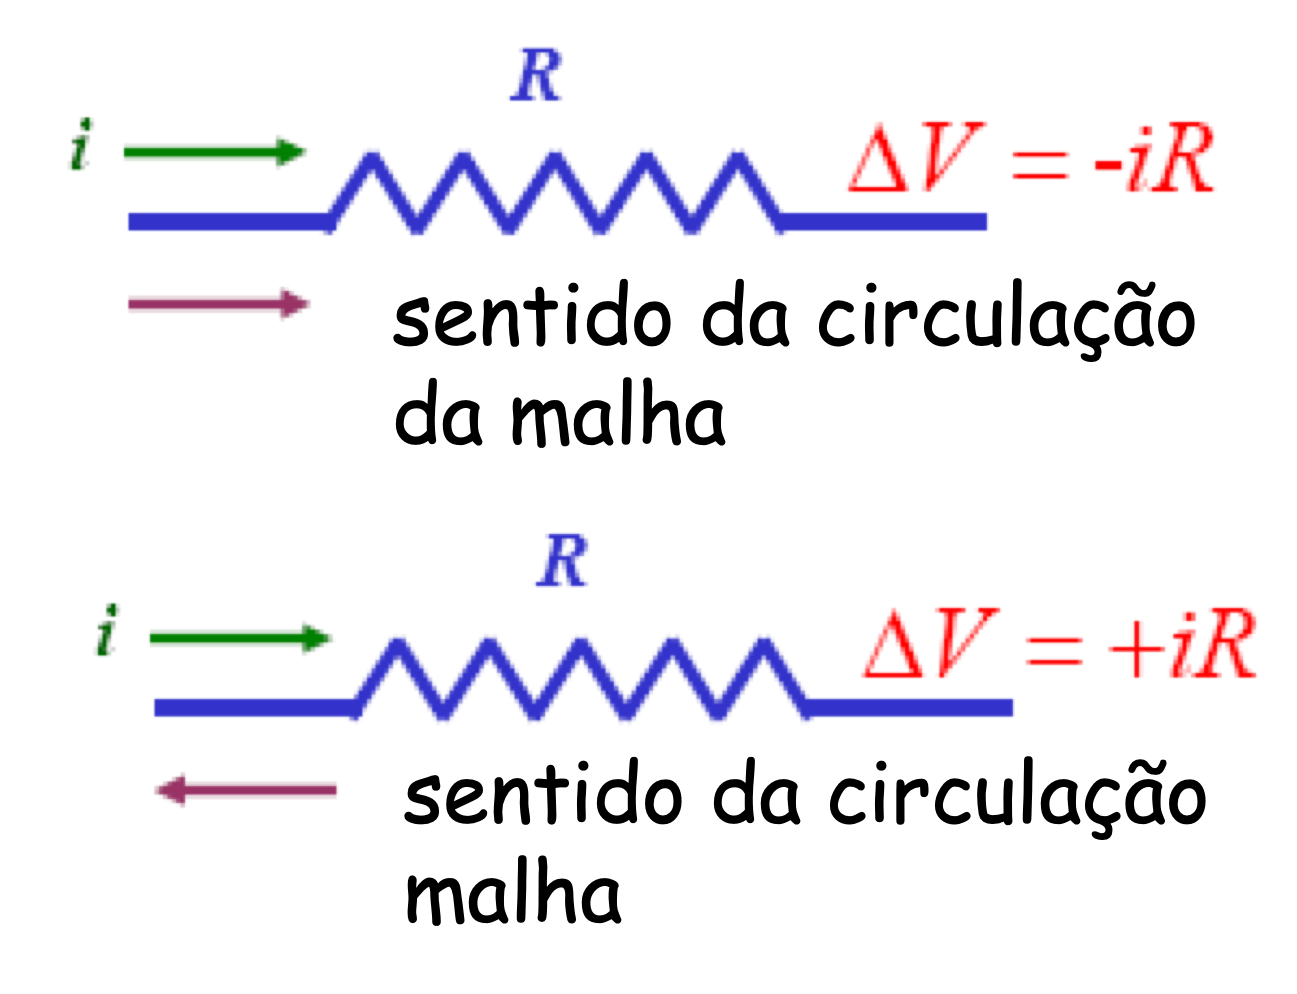
\includegraphics[width=0.8\columnwidth]{Kirk_R.png}
 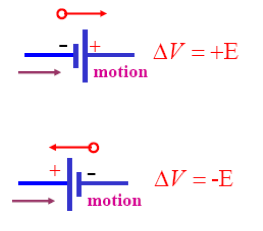
\includegraphics[width=0.8\columnwidth]{Kirk_V.png}
 %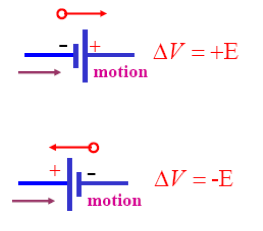
\includegraphics[width=0.3\textwidth]{Kirk_V.png}
    \end{center}
\end{multicols}
}
\mybox{Distribuições de Carga e Correntes}{
    \begin{tabular}{||l|l|l|l||}
        \hline  {\bf Distribuição} &{\bf Carga}&{\bf Campo $\vec{E}$}&{\bf Potencial}\\
        \hline Linear / fio  & \( \mathrm{d}q = \lambda dl \)  & \(\frac{1}{2\pi\varepsilon}\frac{\lambda}{r}\vec{e}_r \) & \\
%        \int \frac{1}{2\pi\varepsilon_0} \frac{\lambda dl}{r^2} \vec{e}_r\) \\
        \hline Superfície & \( \mathrm{d}q = \sigma dA \)  & \(\vec{E} =
        \frac{\sigma}{2 \varepsilon} \vec{e}_{z}$ &\\
%         \frac{1}{4\pi\epsilon_0} \frac{\sigma dA}{r^2} \vec{e}_r \) \\
        \hline Condutor esférico & $\sigma = \frac{Q}{4 \pi R^2}$ & & $\kappa_e \frac{Q}{R}$\\
        \hline
    \end{tabular}
    \\~
    \begin{tabular}{||l|ll||}
        \hline  {\bf Distribuição} & {\bf Campo $\vec{B}$}&\\
        \hline Fio Infinito & \( B = \mu_0 \frac{I}{2 \pi R}\)&\\ 
        \hline Espira Circular & \( B_z = \frac{\mu_0}{2}\frac{I R^2}{(z^2 + R^2)^3/2 }\) & \(z\to0 : B_z = \mu_0 \frac{I}{2 R}\)\\ 
        \hline Solenóide  & \( B = \mu_0 I \frac{N}{l}\)&\\ 
        \hline
    \end{tabular}
}
\mybox{Geometria e Produto Externo}{
    \begin{tabular}{||l|r||}
        \hline Área do Círculo & \( \pi r^2\) \\
        \hline Volume da Esfera & \( \frac{4}{3} \pi r^3\) \\
        \hline Superfície (área exterior) da Esfera & \( 4 \pi r^2\) \\
        \hline
    \end{tabular}\\ 
    \\Produto Externo de vectores como determinante de matriz:
    \begin{equation*}
    \vec{a} \times \vec{b} = \begin{vmatrix}
        \vec{e}_x & \vec{e}_y & \vec{e}_z \\
        a_1 & a_2 & a_3 \\
        b_1 & b_2 & b_3 \\
    \end{vmatrix}
    \end{equation*}
    \begin{equation*}
        |\vec{a} \times \vec{b}| = |\vec{a}| |\vec{b}| \sin(\theta)
    \end{equation*}
}
\mybox{Campo de Indução Magnética $\vec{B}$}{
    Lei de Biot-Savart:
    \begin{equation}
        \vec{B} = \frac{\mu_0}{4 \pi} \frac{q (\vec{v} \times \vec{e}_r) }{r^2} \qquad [\SI{}{\tesla}]
    \end{equation}
    Força de Lorentz:
    \begin{equation}
        \vec{F} = q  \vec{E}  + q \left( \vec{v} \times \vec{B} \right)
    \end{equation}
    Força magnética sobre correntes:
    \begin{equation}
        \vec{F}_{mag} = I \left( \vec{l} \times \vec{B}\right) 
    \end{equation}
    Momento magnético e Torque numa espira:
    \begin{align}
        \vec{\mu}_{mag} &= I  \vec{A}\\
        \vec{\tau}_{mag} &=  \vec{\mu}_{mag} \times \vec{B} \qquad [\SI{}{\newton\meter}]
    \end{align}
    Lei de Ampère:
    \begin{equation}
        \oint \vec{B} \cdot  \mathrm{d}\vec{l} = \mu_0 \sum_i I_i
    \end{equation}
     Fluxo Magnético:
    \begin{equation}
        \Phi_{mag} \equiv \iint_{area} \vec{B} \cdot \mathrm{d}\vec{A} \qquad  [\SI{}{\weber}]= [\SI{}{\tesla\meter\squared}]
    \end{equation}
    Lei de Faraday (Indução Magnética):
    \begin{equation}
        \varepsilon = -\frac{\Phi_{mag}}{\mathrm{d} t} \qquad [\SI{}{\volt}]
    \end{equation}
    Lei de Lenz:\\
    ``A corrente elétrica induzida terá o sentido que se opõe à variação do fluxo que lhe deu origem''.\\
    \\~
    Indutores (Bobines):
    \begin{equation}
        \color{red}
        V_L = - L\frac{\mathrm{d} I}{\mathrm{d} t}
    \end{equation}
     Indutância do solenóide:
    \begin{equation}
        \color{red}
        L = \mu_0 \frac{N^2 A}{l} \qquad [\SI{}{\henry}]
    \end{equation}
}
\mybox{Ferromagnetismo.}{
    Magnetização do Material $\vec{M}$ e Susceptibilidade Magnética $\chi$:
    \begin{equation}
        \vec{M} = \chi_m\frac{\vec{B}_{aplicado}}{\mu_0}
    \end{equation}
    Campo $\vec{H}$, criado pelas correntes \emph{livres}:
    \begin{align}
        \vec{H} &= \frac{\vec{B}}{\mu_0} - \vec{M}\\
        \vec{B} &= (1 + \chi) \mu_0 \vec{H} = \mu_r \mu_0 \vec{H}
    \end{align}
    Lei de Ampère para as correntes \emph{livres}:
    \begin{equation}
        \oint \vec{H} \cdot  \mathrm{d}\vec{l} = \sum_i I_{free}
    \end{equation}
}
%
\mybox{Equações (Leis) de Maxwell.}{
Forma integral
    \begin{tabular}{||l|r||}
        \hline  {\bf Lei} & {\bf Equação }\\
        \hline Gauss para \(\vec{E}\)  & \( \oint \vec{E}\cdot  \mathrm{d}\vec{A}  = \frac{e}{\varepsilon_0} \)\\
        \hline Gauss para \(\vec{B}\)  & \( \oint \vec{B}\cdot  \mathrm{d}\vec{A}  = 0 \)\\
        \hline Faraday  & \( \oint \vec{E} \cdot  \mathrm{d}\vec{l}  = -\frac{\mathrm{d}\Phi_{mag}}{\mathrm{d} t} \)\\
        \hline Ampère-Maxwell  & \( \oint \vec{B} \cdot  \mathrm{d}\vec{l}  = \mu_0 I +\mu_0 \varepsilon_0\frac{\mathrm{d}\Phi_{ele}}{\mathrm{d} t} \)\\
        \hline
    \end{tabular} 
}
\mybox{Dinâmica}{
    Força e Aceleração (2ª Lei de Newton):
    \begin{equation*}
        \vec{F}= m \vec{a} \qquad [\SI{}{\newton}]
    \end{equation*}
    Trabalho produzido por uma Força no trajecto \( A \to B\):
    \begin{equation*}
        W = \int_A^B \vec{F} \cdot  \vec{dl}
    \end{equation*}
    Momento angular:
    \begin{equation*}
        \vec{L} =  \vec{r} \times m \vec{v} \qquad [\SI{}{\kilogram\meter\squared\per\second}]
    \end{equation*}
    Força centrípeda:
    \begin{equation*}
        F_{cent} =  m \frac{v^2}{r} 
    \end{equation*}
}

\end{multicols}
\mybox{Circuitos em Corrente Contínua (DC)}{
    \begin{tabular}{||l|l|l|l|l||}
        \hline   &{\bf $t=0^+$} &{\bf $t\to\infty$} &{\bf Carga} &{\bf Descarga}\\
        \hline C  & $V_C = 0$ (CC) & $I_C =0 $ (CA) &$V_C(t) = V_{f} (1-e^{-t/\tau_C}) $ &$V_C(t) = V_{0} e^{-t/\tau_C}$\\ 
        \hline L  & $I_L(t=0^-) = I_L(t=0^+)$ & $V_L =0 $ (CC)  &$I(t) = I_{f} (1-e^{-t/\tau_L})$ &$I_L(t) = I_{0} e^{-t/\tau_L}$\\ 
        \hline
    \end{tabular}
    \\~
    $\tau_C = RC$, $\tau_L = \frac{L}{C} \; [\mathrm{s}]$. CC: Curto-Circuito. CA: Circuito Aberto
}

% End the document
\end{document}

